
\documentclass[article]{IEEEtran}
\usepackage[a5paper, margin=10mm, onecolumn]{geometry}

\usepackage{tfrupee} 
\setlength{\headheight}{1cm} 
\setlength{\headsep}{0mm}       
\usepackage{multicol}
\usepackage{gvv-book}
\usepackage{gvv}
\usepackage{cite}
\usepackage{amsmath,amssymb,amsfonts,amsthm}
\usepackage{algorithmic}
\usepackage{graphicx}
\usepackage{textcomp}
\usepackage{xcolor}
\usepackage{txfonts}
\usepackage{listings}
\usepackage{enumitem}
\usepackage{mathtools}
\usepackage{gensymb}
\usepackage{comment}
\usepackage[breaklinks=true]{hyperref}
\usepackage{tkz-euclide} 
\usepackage{listings}

\def\inputGnumericTable{}                                 
\usepackage[latin1]{inputenc}                                
\usepackage{color}                                            
\usepackage{array}                                            
\usepackage{longtable}                                       
\usepackage{calc}                                             
\usepackage{multirow}                                         
\usepackage{hhline}                                           
\usepackage{ifthen}                                           
\usepackage{lscape}
\begin{document}
	\title{9.6.2}
	\author{EE25BTECH11052 - Shriyansh Kalpesh Chawda}
	\maketitle
\textbf{Question}\\
Find the area of the circle $4x^{2} + 4y^{2} = 9$ which is interior to the parabola $x^{2} = 4y.$\\
\textbf{Solution}\\
The conic parameters for the two curves can be expressed as follows:\\
For the circle $4x^2 + 4y^2 - 9 = 0$:
\begin{align}
\mathbf{V_1} = \myvec{4 & 0 \\ 0 & 4}, \mathbf{u_1} = \myvec{0 \\ 0}, f_1 = -9. 
\end{align}
For the parabola $x^2 - 4y = 0$:
\begin{align}
\mathbf{V_2} = \myvec{1 & 0 \\ 0 & 0}, \mathbf{u_2} = \myvec{0 \\ -2}, f_2 = 0. 
\end{align}
The intersection of two conics with parameters $\mathbf{V_i}$, $\mathbf{u_i}$, $f_i$, i = 1, 2 is defined as:
\begin{equation}
	\mathbf{x}^\top(\mathbf{V_1} + \mu\mathbf{V_2})\mathbf{x} + 2(\mathbf{u_1} + \mu\mathbf{u_2})^\top\mathbf{x} + (f_1 + \mu f_2) = 0 
\end{equation}
For a degenerate conic, the determinant of the quadratic part's matrix must be zero.
\begin{align}
&\det(\mathbf{V_1} + \mu\mathbf{V_2}) = 0 \\
&\det\left(\myvec{4 & 0 \\ 0 & 4} + \mu\myvec{1 & 0 \\ 0 & 0}\right) =
\begin{vmatrix}
	4+\mu & 0 \\
	0 & 4
\end{vmatrix}
 = 4(4+\mu) = 0 \\
&\mu = -4
\end{align}
Substituting $\mu = -4$ in (3) :
\begin{align} 
&\mathbf{x}^\top( \mathbf{V_1} - 4\mathbf{V_2} )\mathbf{x} + 2( \mathbf{u_1} - 4\mathbf{u_2} )^\top\mathbf{x} + ( f_1 - 4f_2 ) = 0 \\
&\mathbf{x}^\top\left( \myvec{4 & 0 \\ 0 & 4} - 4\myvec{1 & 0 \\ 0 & 0} \right)\mathbf{x} + 2\left( \myvec{0 \\ 0} - 4\myvec{0 \\ -2} \right)^\top\mathbf{x} + ( -9 - 4(0) ) = 0 \\
&\mathbf{x}^\top \myvec{0 & 0 \\ 0 & 4} \mathbf{x} + 2 \myvec{0 \\ 8}^\top \mathbf{x} - 9 = 0 
\end{align}
Letting $\mathbf{x} = \myvec{x \\ y}$, the equation becomes:
\begin{align} \myvec{x & y} \myvec{0 & 0 \\ 0 & 4} \myvec{x \\ y} + 2 \myvec{0 & 8} \myvec{x \\ y} - 9 = 0 \end{align}
\begin{align} \implies 4y^2 + 16y - 9 = 0 \end{align}
Solving for y yields $y = 1/2$ and $y = -9/2$. For the area to be interior to the parabola $x^2 = 4y$, we must have $y \ge 0$. Therefore, the intersection occurs at the line $y = 1/2$. Substituting $y = 1/2$ into the parabola's equation:
\begin{align} x^2 = 4(1/2) = 2 \implies x = \pm\sqrt{2}. \end{align}
Hence, the points of intersection are:
\begin{align} 
\mathbf{a_1} = \myvec{\sqrt{2} \\ 1/2}, \mathbf{a_2} = \myvec{-\sqrt{2} \\ 1/2}
\end{align}
The desired area of the region is given by:
\begin{align} A = \int_{-\sqrt{2}}^{\sqrt{2}} \left( \sqrt{\frac{9}{4} - x^2} - \frac{x^2}{4} \right) dx \
\end{align}
Due to symmetry,
\begin{align}
	&= 2 \left[ \int_{0}^{\sqrt{2}} \sqrt{\frac{9}{4} - x^2} \, dx - \int_{0}^{\sqrt{2}} \frac{x^2}{4} \, dx \right] \\
	\intertext{The first integral uses the standard formula for $\sqrt{a^2-x^2}$ (from trig substitution).}
	\int_{0}^{\sqrt{2}} \sqrt{\frac{9}{4} - x^2} \, dx &= \frac{\sqrt{2}}{4} + \frac{9}{8}\sin^{-1}\left(\frac{2\sqrt{2}}{3}\right) \\
	\intertext{The second integral uses the simple power rule.}
	\int_{0}^{\sqrt{2}} \frac{x^2}{4} \, dx &= \frac{\sqrt{2}}{6} \\
	\intertext{Substituting these results back:}
	A &= 2 \left[ \left( \frac{\sqrt{2}}{4} + \frac{9}{8}\sin^{-1}\left(\frac{2\sqrt{2}}{3}\right) \right) - \frac{\sqrt{2}}{6} \right] \\
	&= \frac{\sqrt{2}}{6} + \frac{9}{4}\sin^{-1}\left(\frac{2\sqrt{2}}{3}\right)
\end{align}
\begin{figure}[H]
	\centering
	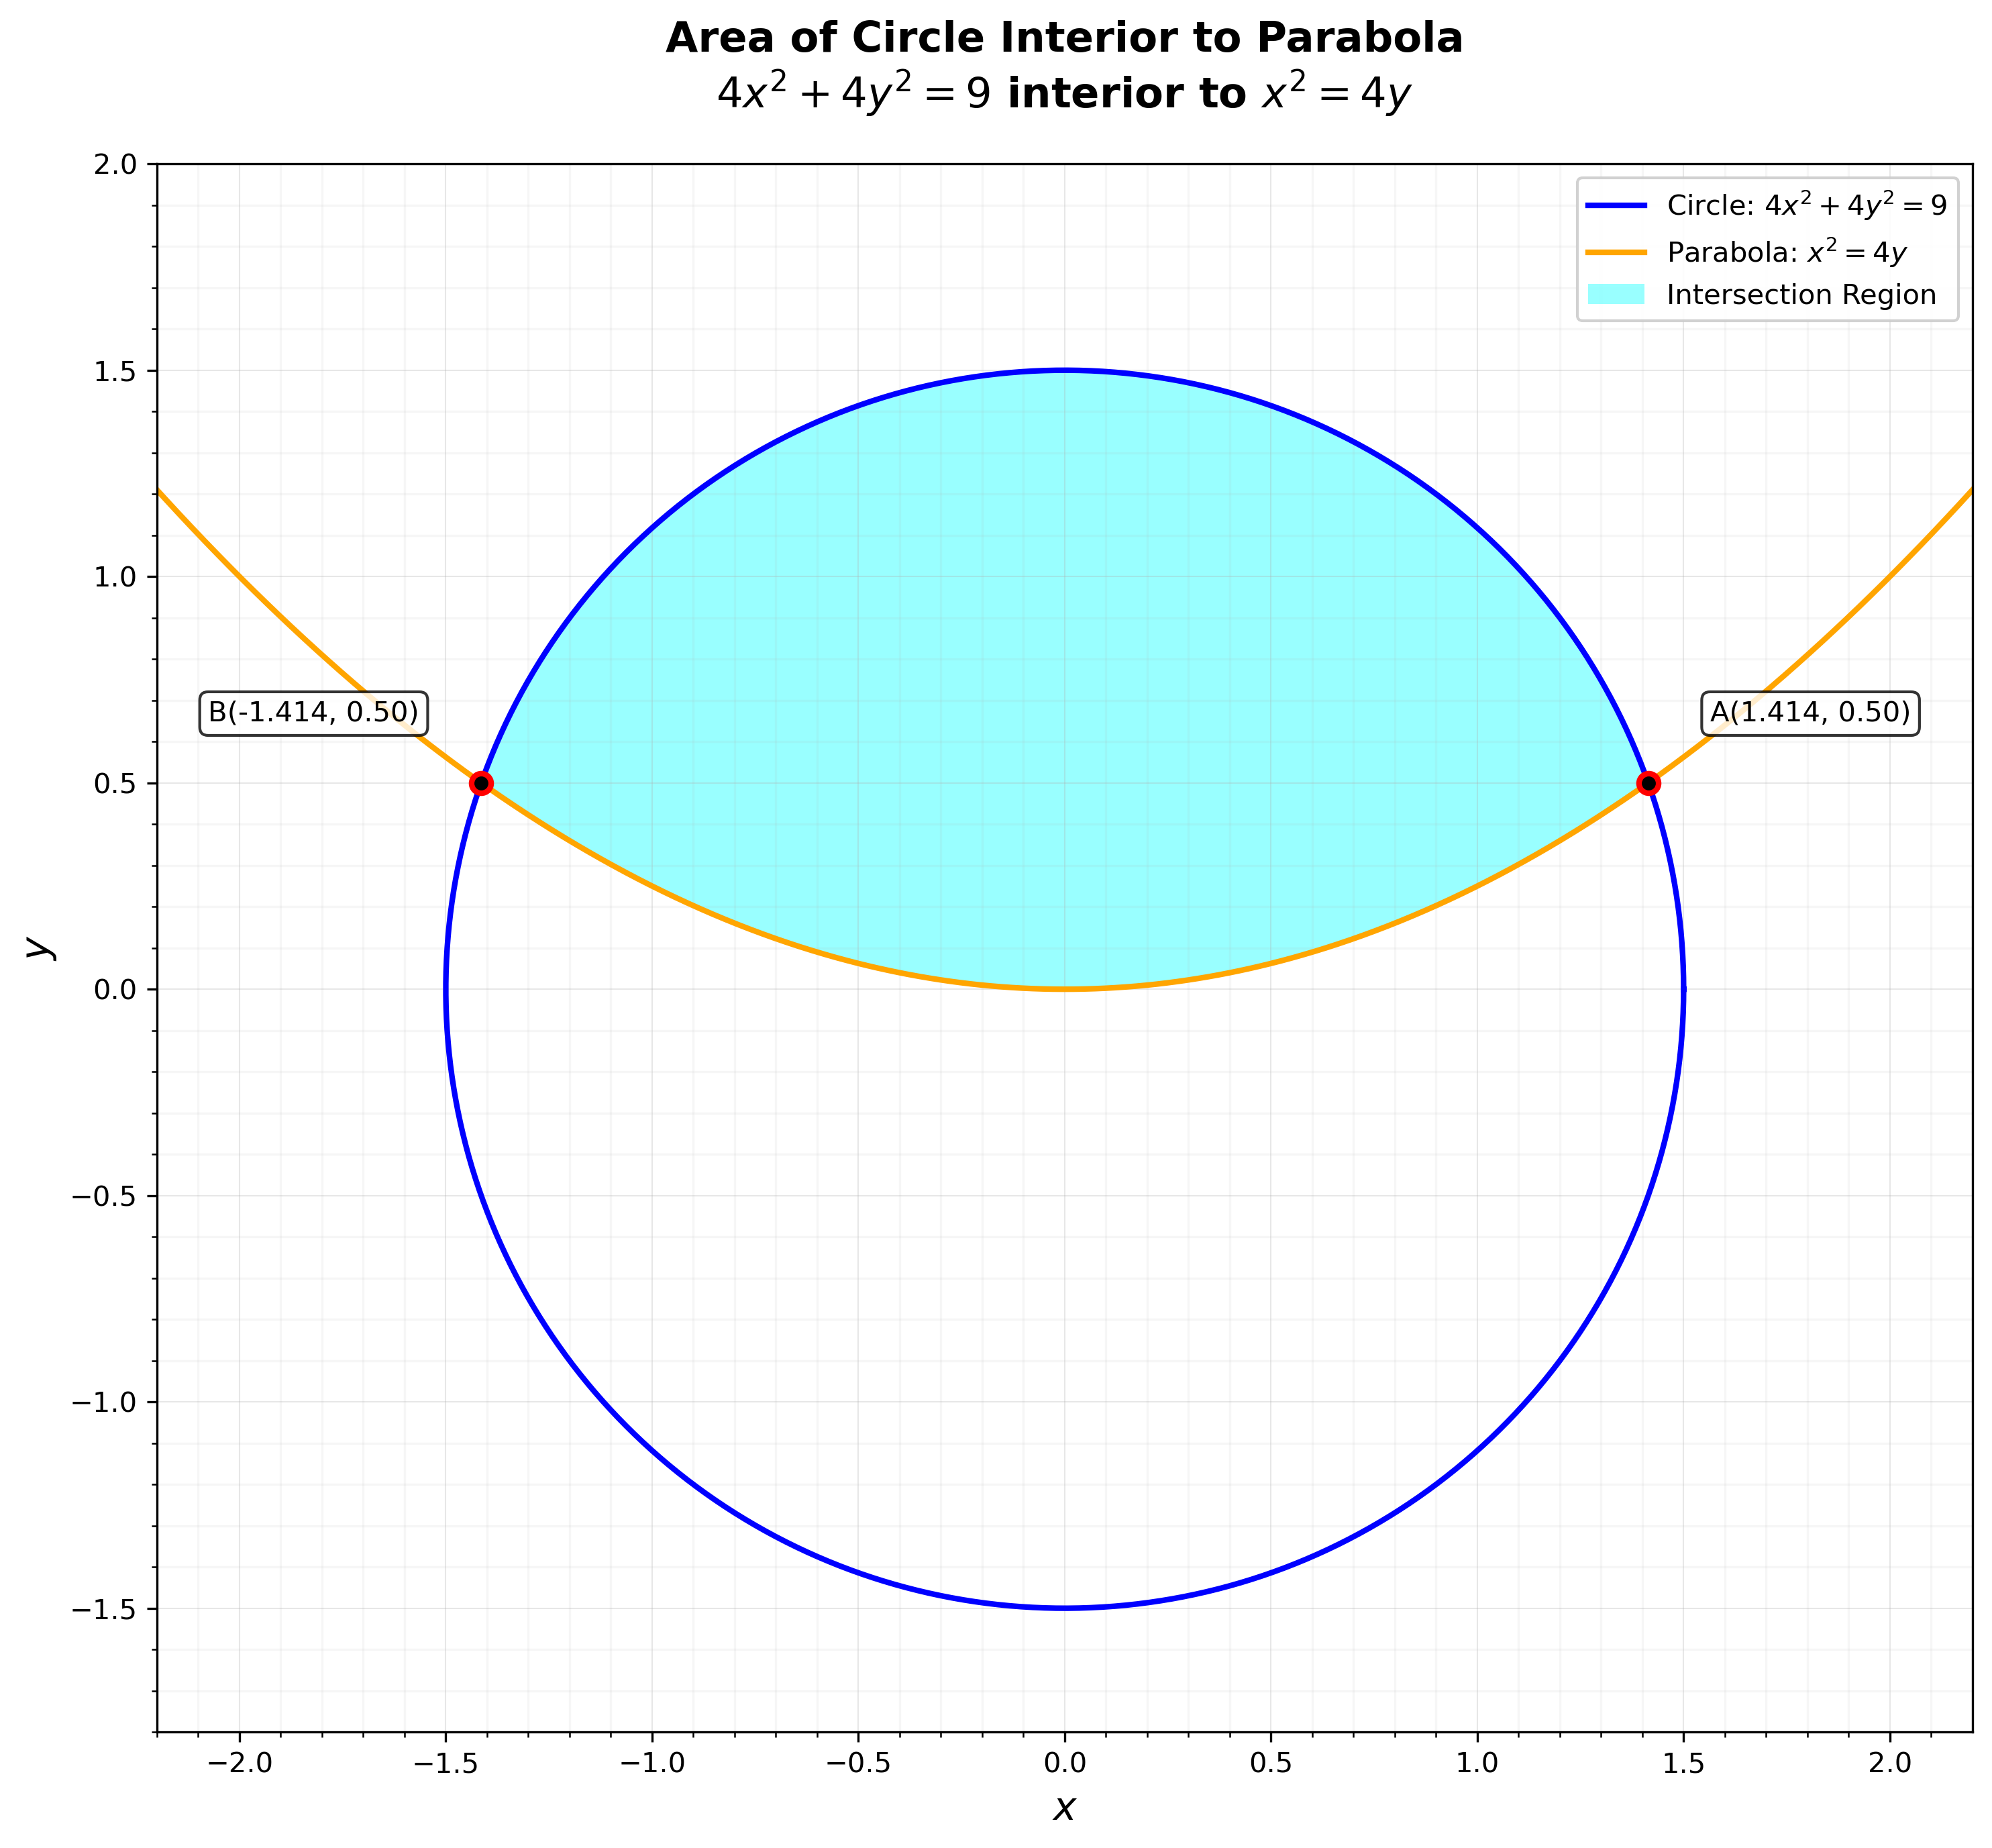
\includegraphics[width=1\linewidth]{figs/area_plot}
\end{figure}


\end{document}